%%%%%%%%%%%%%%%%%%%%%%%%%%%%%%%%%%%%%%%%%%%%%%%%%%%%%%%%%%%%%%%
%
% Welcome to Overleaf --- just edit your LaTeX on the left,
% and we'll compile it for you on the right. If you open the
% 'Share' menu, you can invite other users to edit at the same
% time. See www.overleaf.com/learn for more info. Enjoy!
%
%%%%%%%%%%%%%%%%%%%%%%%%%%%%%%%%%%%%%%%%%%%%%%%%%%%%%%%%%%%%%%%
%%%%%%%%%%%%%%%%%%%%%%%%%%%%%%%%%%%%%%%%%%%%%%%%%%%%%%%%%%%%%%%%%%%%%%%%
%% Skip to the "\begin{document}" line below to see the visible text. %%
%% Compare the left and right-hand panes to compare what you type and %%
%% how it appears when typeset.                                       %%
%%                                                                    %%
%% ***** Type answers after the next line that looks like this  ***** %%
%%%%%%%%%%%%%%%%%%%%%%%%%%%%%%%%%%%%%%%%%%%%%%%%%%%%%%%%%%%%%%%%%%%%%%%%
\documentclass[12pt]{article}
\usepackage{mathrsfs}
\usepackage{amsmath,amssymb}
\usepackage{graphicx}
\usepackage[utf8]{inputenc}
\usepackage{tkz-berge}
\usepackage{pgf}
\usepackage{xcolor}
\usepackage{algorithm}
\usepackage{caption}
\usepackage{multicol}
\usepackage{array}
\usepackage[noend]{algpseudocode}
\newcommand{\Term}{Winter 2019}
\newcommand{\Course}{104.272 Discrete Mathematics}

\newcommand{\Assignment}{1. Exercise}
\newcommand{\DueDate}{ 16 October, 2019 }

\usepackage[body={6in,9in}]{geometry}



\begin{document}
Hugo \textit{Rincon Galeana}
\begin{center}

\textbf{TU Wien, \Term} \\
\textbf{\Course} (Professor Gittenberger) \\
\textbf{\Assignment, Due \DueDate}
\end{center}


%%%%%%%%%%%%%%%%%%%%%%%%%%%%%%%%%%%%%%%%%%%%%%%%%%%%%%%%%%%%%%%%%%%%%%%%
%% *****      Type your answers after the "\soln" commands      ***** %%
%%%%%%%%%%%%%%%%%%%%%%%%%%%%%%%%%%%%%%%%%%%%%%%%%%%%%%%%%%%%%%%%%%%%%%%%
\begin{enumerate}

\item A simple undirected graph is called cubic if each of its vertices has degree $3$.
    \begin{enumerate}
        \item Find a cubic graph with 6 vertices!
        
        \vspace{1em}
        A triangular prism
        
\begin{center}

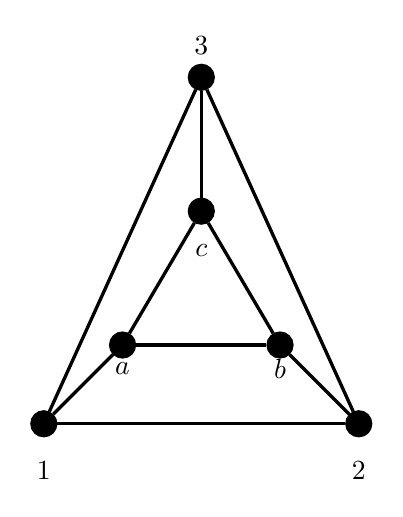
\begin{tikzpicture}

     \node[shape=circle,draw=black, fill = black] (B1)  at (-1,-1){};
     \node (B1n)  at (-1,-1.3){$a$};
     \node[shape=circle,draw=black, fill = black] (R1)  at (1,-1){};
     \node (R1n)  at (1,-1.3){$b$};
     \node[shape=circle,draw=black, fill = black] (B2)  at (0,0.7){};
     \node (B2n)  at (0,0.2){$c$};

     
    \node[shape=circle,draw=black, fill = black] (A1)  at (-2,-2){};
     \node (A1n)  at (-2,-2.6){$1$};
     \node[shape=circle,draw=black, fill = black] (C1)  at (2,-2){};
     \node (C1n)  at (2,-2.6){$2$};
     \node[shape=circle,draw=black, fill = black] (A2)  at (0,2.4){};
     \node (A2n)  at (0,2.8){$3$};

 
     

     \draw [draw=black,-,very thick] (B1) to  (R1);
     \draw [draw=black,-,very thick] (R1) to  (B2);
     \draw [draw=black,-,very thick] (B2) to  (B1);

     
    \draw [draw=black,-,very thick] (A1) to  (C1);
     \draw [draw=black,-,very thick] (C1) to  (A2);
     \draw [draw=black,-,very thick] (A2) to  (A1);
    
     
     \draw [draw=black,-,very thick] (A1) to  (B1);
     \draw [draw=black,-,very thick] (R1) to  (C1);
     \draw [draw=black,-,very thick] (B2) to  (A2);

     

     \end{tikzpicture}


     \end{center}
     
     \item Is there a cubic graph with an odd number of vertices?
     \vspace{1em}
     
No, let's assume by contradiction that there exists a cubic graph
     $G=(V,E)$ such that $\lvert V \rvert = 2 \cdot k +1 $ for some $k \in \mathbb{N}$. Let us consider $s = \sum\limits_{v \in V} \delta (v)$. Since $G$ is a cubic graph, it follows from definition that $s = 3 \cdot \lvert V \rvert = 2 \cdot (3k)+1$. It also follows from the handshaking lemma that $s = 2 \cdot \lvert E  \rvert$. It follows that $\lvert E \rvert = 3k + \frac{1}{2}$, which contradicts that $\lvert E \rvert$ should be a natural number.
     It follows from contradiction that $\lvert V \rvert$ is not odd.
     
     \item Prove that for all $n\geq 2$ there exists a cubic graph with $2n$ vertices!
     \vspace{1em}
     
  For the case $n = 2$, consider the complete simple graph $K_4$ with 4 vertices and exactly one edge for each pair of vertices. $K_4$ is cubic.
     
     Now, lets consider $n>2$. Consider $C_n$ a cycle of $n$ vertices $C_n = (v_0, v_1, \ldots, v_{n-1},v_0)$ , and $C'_n$ another cycle of $n$ vertices $C'_n = (w_0,w_1,\ldots,w_{n-1},w_0)$ such that $V(C_n) \cap V(C'_n) = \varnothing$.
     
     We define $G_n$ as follows: 
     
     \begin{itemize}
         \item $V(G_n) = V(C_n) \cup V(C'_n)$
         \item $E(G_n) = E(C_n) \cup E(C'_n) \cup \{ (v_i,w_i) \vert \; v_i \in V(C_n), w_i \in V(C'_n) \}$
     \end{itemize}
     
     Let $v$ be a vertex in $G_n$. Let's assume without loss of generality that $v = v_r $ for some $r \in \{0,\ldots, n-1\}$. From construction, $v = v_r$ is adjacent to $v_{r-1 \textrm{ mod } n}$, $v_{r+1 \textrm{ mod } n} $ and $w_r$, therefore $\delta(v)=3$.
     
     The proof is symmetrical when $v = w_r$ for some $r \in \{0,\ldots,n-1 \}$.
     
     Informally $G_n$ is an $n$-prism. 
     \begin{center}
         

    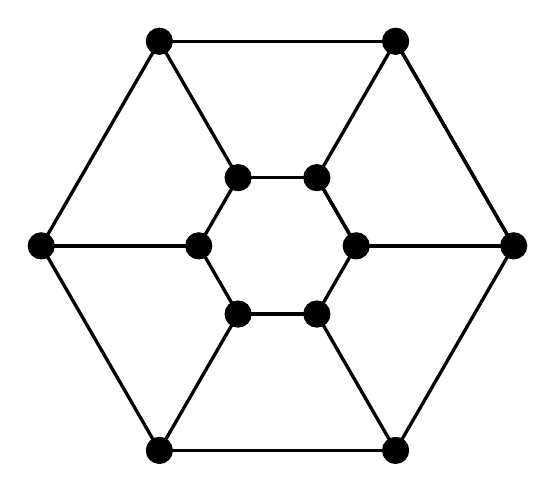
\begin{tikzpicture}
    \foreach \a in {0, 60,...,300}
        \node[shape=circle,draw=black, fill = black] at (\a:1){};
    \foreach \a in {0,60,...,360}
        \draw [draw=black,-,very thick] (\a:1) to  (\a+60:1);
    
    \foreach \a in {0, 60,...,300}
        \node[shape=circle,draw=black, fill = black] at (\a:3){};
    \foreach \a in {0,60,...,360}
        \draw [draw=black,-,very thick] (\a:3) to  (\a+60:3);
    \foreach \a in {0,60,...,300}
        \draw [draw=black,-,very thick] (\a:1) to  (\a:3);
    
    \end{tikzpicture}
\end{center}
     
    \end{enumerate}
    
\item Use a suitable graph theoretical model to solve the following problems:
    \begin{enumerate}
        \item Show that in every city at least two of its inhabitants have the same number of neighbours!
        
        Consider a graph $G$ with a set of vertices $V = \{v_1, \ldots ,v_n \}$ such that $n$ is the number of inhabitants in the city. Let us assume that there is a bijective mapping that assigns a number from $\{1,\ldots,n\}$ to each of the inhabitants. 
        
        In our model, vertex $v_k$ represents the inhabitant associated with number $k$.
        Now, we can define the edges for our graph. $E = \{(v_i,v_j) \vert \; v_i, v_j \in V  \}$ and the inhabitant with assigned number $i$ is neighbor to the inhabitant with assigned number $j$. 
        
        For simplicity we will not consider multiple neighbor relations nor will we consider that an inhabitant is neighbor to himself.
        
        The problem translates to showing that in a simple graph $G$, there exist two vertices $v \neq w$ such that $\delta(v) = \delta(w)$.
        
        Assume by contradiction that there are no such two vertices $v,w$. Since $G$ is a simple graph, this implies that $\delta: V(G) \rightarrow \{0,\ldots,n-1\}$ is an injective mapping. Since $V(G)$ is finite and $\vert V(G) \vert =\vert \{0,\ldots,n-1\} \vert=n $, then $\delta :V(G) \rightarrow \{0,\ldots,n-1\}$ is a bijection. Therefore, there exists $v$ such that $\delta(v)=0$ and there exists $w$ such that $\delta(w)=n-1$. From $\delta(v)=0$ we get that $(v,w) \notin E$. From $\delta(w)=n-1$, we get that $(v,w) \in E$. This is a contradiction. Therefore $\delta$ is not injective. 
        
        Since $\delta$ is not injective, then there exist $v\neq w$ such that $\delta(v) = \delta (w)$. Translating our model, we show that inhabitant with assigned vertex $v$ has the same number of neighbours as inhabitant with assigned vertex $w$.
        
        \item A group of friends goes (separately) on holidays. Each of them sends a postcard to three members of the group. When is it possible that every member of the group receives postcards from precisely those friends to whom he/she sent postcards?
        
        We will consider a graph $G = (V,E)$ with a set of vertices $V$ that represents the group of friends as in the previous solution. The set of edges $E$ is given by pairs $(v,w)$ where the friend represented by vertex $v$ sent a postcard to the friend represented by $w$.
        
        Since we are only interested in modeling the case where each friend receives a postcard from the friends they send the postcards, then we do not need directed edges.
        
        This model translates to determine which are the graphs such that each vertex has degree 3. This is the definition of cubic graphs.
        
        Therefore the situation described in the problem is only achievable when the graph defined previously is a cubic graph.
    \end{enumerate}
    
    \item Are the following two graphs isomorphic?
    
    \includegraphics[width=0.9\textwidth]{graficast1.JPG} \\
    
    Yes, consider the following graph isomorphism.
    
    $\mu(1) = C$;
    $\mu(2) = \beta$;
    $\mu(3) = A$;
    $\mu(4) = \delta$;
    $\mu(a)= \alpha$;
    $\mu(d)= D$;
    $\mu(c) = \gamma$;
    $\mu (b) =\beta$;
    
    \item 
        \begin{enumerate}
        \item Compute the number of walks of length $\ell$ from $i$ to $j$ in the graph 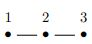
\includegraphics{t3.JPG}
        
        \vspace{1em}
        Let us notice that a walk of length $\ell$ is a sequence of vertices $(w_0,w_1, \ldots, w_{\ell})$ such that $w_i$ is adjacent to $w_{i+1}$ for any $i$. From definition, it follows that if $w_j = v_1$ or $w_j = v_3$, then $w_{j+1} = v_2$ since both vertices $v_1$ and $v_3$ are only adjacent to $v_2$.
        
        First let us consider walks that begin and end in $v_2$. Consider a walk $W = (w_0 = v_2, w_1, \ldots, w_{\ell}=v_2)$. Inductively, every vertex $v_i$ such that $i$ is even, must be equal to $v_2$ (from the previous observation). Notice also that any $v_j$ such that $j$ is odd, must be equal to either $v_1$ or $v_3$. Therefore, we may only have 2 different vertex possibilities per each of the vertices $v_j$ with $j$ odd. The rest of the vertices are forced to be equal to $v_2$. Since we have exactly $\ell /2 $ odd vertices, then we have exactly $\displaystyle 2^{\ell/2}$ possible walks.
        
        Let us now consider a walk $W =(w_0, w_1, \ldots, w_{\ell}= v_2)$ that either begin in $v_1$ or $v_3$ and end in $v_2$. From a previous observation we get that $w_1 = v_2$. Notice that since $w_0$ is fixed and $(w_1 = v_2, \ldots, w_{ell}= v2)$, then there is the same amount of walks of length $\ell$ of this kind as the walks of lenght $\ell-1$ that begin and end in $v_2$. Therefore, in this case there are $2^{\ell-1}$ possible walks.
        
        Notice that for walks that begin in $v_2$ and end in either $v_1$ or $v_3$, the computation is symmetrical, and therefore there are $2^{\ell-1}$ possible walks.
        
        Now let us consider walks that do not begin nor end in $v_2$. In such case, then a walk $W=(w_0, \ldots, w_{\ell})$ must begin in either $v_1 $ or $v_3$ and end in either $v_1$ or $v_3$. In such case, notice that $w_1 = v_2$ and $w_{\ell -1}= v_2. $ It follows that $(w_1, \ldots , w_{\ell -1})$ is a walk that begins and ends with $v_2$ of length $\ell-2$. Since $w_0$ and $w_{\ell}$ are fixed, then the amount of walks that do not begin nor end in $v_2$ can be computed as $2^{\ell-2}$.
        
        This completes the computation for all walks in the given graph.
        
        \item How could you use the adjacency matrix to compute the number of triangles (i.e, the cycles of length three) in a (loopless) graph? Perform the computation for two graphs of your choice on four vertices.
        
        
        
        
        First, we will show how to find all triangles in a graph, then we will give a simple solution to just compute the number of triangles. Since we are only considering undirected graphs, we can only use the upper right triangular adjacency matrix.
        
       \begin{algorithm}
            \caption{Algorithm for finding triangles in simple undirected graphs}\label{3cycles}
            \begin{algorithmic}
            \Procedure{3-Cycles}{}
            \State $i\gets 1$
            \State $C\gets \varnothing$
            \For{$i<n-1; i\gets i+1$} 
                \State $j\gets i+1$
                \For{$j<n; j\gets j+1$}
                    \If{$A_{ij} \neq \infty$}
                        \State $k \gets j+1$
                        \For{$k < n+1; k \gets k+1$}
                            \If{$A_{ik} \neq \infty$ \textbf{and} $A_{jk} \neq \infty$}
                                \State $C \gets C \cup \{(v_i,v_j,v_k)\}$
                            \EndIf
                        \EndFor
                    \EndIf
                \EndFor
            \EndFor
            \Return $C$
\EndProcedure
\end{algorithmic}
\end{algorithm}

This algorithm iterates first over the vertices in order to explore all edges, and then for every edge, it iterates over the rest of vertices in order to find vertices that are adjacent to both ends of the given edge. It has a complexity of $\mathcal{O}(n^3)$, that makes it optimal since the any complete graph has $\mathcal{O}(n^3)$ triangles.

\addtolength{\tabcolsep}{1em}
\begin{tabular}{ m{5cm}  m{3cm} m{3cm} }
\textbf{Graph figures}
&
        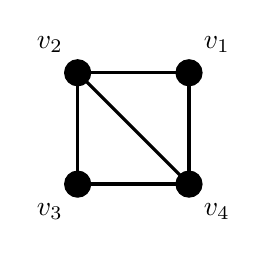
\begin{tikzpicture}
    \foreach \a in {1, 2,...,4}
        {\node[shape=circle,draw=black, fill = black] at (\a*90-45:1){};
        \node at (\a*90-45:1.5){$v_{\a}$};}
    \foreach \a in {-45,45,...,315}
        \draw [draw=black,-,very thick] (\a:1) to  (\a+90:1);
    \draw [draw=black,-,very thick] (135:1) to  (-45:1);
    \end{tikzpicture}
       
&        
        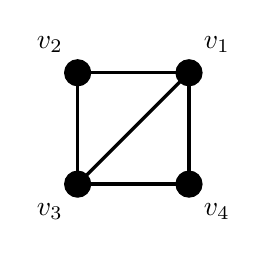
\begin{tikzpicture}
    \foreach \a in {1, 2,...,4}
        {\node[shape=circle,draw=black, fill = black] at (\a*90-45:1){};
        \node at (\a*90-45:1.5){$v_{\a}$};}
    \foreach \a in {-45,45,...,315}
        \draw [draw=black,-,very thick] (\a:1) to  (\a+90:1);

    \draw [draw=black,-,very thick] (-135:1) to  (45:1);
    \end{tikzpicture}

\\
&
    Graph $G_1$  &   Graph $G_2$\\
    \\
    \textbf{Adjacency matrices} &
     $\begin{matrix}
                & v_1 & v_2 & v_3    & v_4  \\
            v_1 & 0   & 1   & \infty & 1 \\
            v_2 & 1   & 0   & 1      & 1 \\
            v_3 & \infty & 1 & 0 & 1\\
            v_4 & 1 & 1 & 1 & 0 \\
    \end{matrix}$
    
   &
   
        $\begin{matrix}
                & v_1 & v_2 & v_3    & v_4  \\
            v_1 & 0   & 1   &  1 & 1 \\
            v_2 & 1   & 0   & 1      & \infty \\
            v_3 & 1 & 1 & 0 & 1\\
            v_4 & 1 & \infty & 1 & 0 \\
    \end{matrix}$ \\
    
    \\
    
    \textbf{Runs} &
    $\begin{matrix}
            & v_1 & v_2 & v_3    & v_4  \\
            \textrm{\textcolor{red}{$v_1$}} & 0   & 1   & \infty & 1 \\
            v_2 & 1   & 0   & 1      & 1 \\
            v_3 & \infty & 1 & 0 & 1\\
            v_4 & 1 & 1 & 1 & 0 \\
    \end{matrix}$
    
   &
   
        $\begin{matrix}
            & v_1 & v_2 & v_3    & v_4  \\
            \textrm{\textcolor{red}{$v_1$}} & 0   & 1   &  1 & 1 \\
            v_2 & 1   & 0   & 1      & \infty \\
            v_3 & 1 & 1 & 0 & 1\\
            v_4 & 1 & \infty & 1 & 0 \\
    \end{matrix}$ \\
    \\
    
    $C_1= \varnothing; \; C_2 = \varnothing$ &
    $\begin{matrix}
            & v_1 & v_2 & v_3    & v_4  \\
            \textbf{\textcolor{red}{$v_1$}} & 0   & \textbf{\textcolor{green}{$1$}}   & \infty & 1 \\
            v_2 & 1   & 0   & 1      & 1 \\
            v_3 & \infty & 1 & 0 & 1\\
            v_4 & 1 & 1 & 1 & 0 \\
    \end{matrix}$
    
   &
   
        $\begin{matrix}
            & v_1 & v_2 & v_3    & v_4  \\
            \textrm{\textcolor{red}{$v_1$}} & 0   &  \textrm{\textcolor{green}{$1$}}   &  1 & 1 \\
            v_2 & 1   & 0   & 1      & \infty\\
            v_3 & 1 & 1 & 0 & 1\\
            v_4 & 1 & \infty & 1 & 0 \\
    \end{matrix}$ \\
    
    \\
    
       $C_1= \{(v_1,v_2,v_4)\}; \; C_2 = \{(v_1,v_2,v_3)\}$ &
    $\begin{matrix}
            & v_1 & v_2 & v_3    & v_4  \\
            \textbf{\textcolor{red}{$v_1$}} & 0   & \textbf{\textcolor{green}{$1$}}   & \infty & \textbf{\textcolor{orange}{$1$}} \\
            v_2 & 1   & 0   & 1      & 1 \\
            v_3 & \infty & 1 & 0 & 1\\
            v_4 & 1 & 1 & 1 & 0 \\
    \end{matrix}$
    
   &
   
        $\begin{matrix}
            & v_1 & v_2 & v_3    & v_4  \\
            \textrm{\textcolor{red}{$v_1$}} & 0   &  \textrm{\textcolor{green}{$1$}}   &  \textbf{\textcolor{orange}{$1$}} & 1 \\
            v_2 & 1   & 0   & 1      & 0\\
            v_3 & 1 & 1 & 0 & 1\\
            v_4 & 1 & 0 & 1 & 0 \\
    \end{matrix}$ \\
    \\
    
    $C_1= \{(v_1,v_2,v_4)\};$   $C_2 = \{(v_1,v_2,v_3),(v_1,v_2,v_4)\}$ &
    $\begin{matrix}
            & v_1 & v_2 & v_3    & v_4  \\
            v_1 & 0   & 1   & 0 & 1 \\
            \textbf{\textcolor{red}{$v_2$}} & 1   & 0   & 1      & 1 \\
            v_3 & 0 & 1 & 0 & 1\\
            v_4 & 1 & 1 & 1 & 0 \\
    \end{matrix}$
    
   &
   
        $\begin{matrix}
            & v_1 & v_2 & v_3    & v_4  \\
            \textrm{\textcolor{red}{$v_1$}} & 0   &  \textrm{\textcolor{green}{$1$}}   &  1 & \textbf{\textcolor{orange}{$1$}} \\
            v_2 & 1   & 0   & 1      & 0\\
            v_3 & 1 & 1 & 0 & 1\\
            v_4 & 1 & 0 & 1 & 0 \\
    \end{matrix}$ \\
    \\
    
    
    
    
\end{tabular}
\begin{tabular}{ m{5cm}  m{3cm} m{3cm} }
$C_1= \{(v_1,v_2,v_4)\};$   $C_2 = \{(v_1,v_2,v_3),(v_1,v_2,v_4)\}$ &
    $\begin{matrix}
            & v_1 & v_2 & v_3    & v_4  \\
            v_1 & 0   & 1   & 0 & 1 \\
            \textbf{\textcolor{red}{$v_2$}} & 1   & 0   & \textbf{\textcolor{green}{$1$}}      & 1 \\
            v_3 & 0 & 1 & 0 & 1\\
            v_4 & 1 & 1 & 1 & 0 \\
    \end{matrix}$
    
   &
   
        $\begin{matrix}
            & v_1 & v_2 & v_3    & v_4  \\
            v_1 & 0   &  1   &  1 & 1 \\
            \textbf{\textcolor{red}{$v_2$}} & 1   & 0   & 1      & 0\\
            v_3 & 1 & 1 & 0 & 1\\
            v_4 & 1 & 0 & 1 & 0 \\
    \end{matrix}$ \\
    \\
    
    $C_1= \{(v_1,v_2,v_4),(v_2,v_3,v_4)\};$   $C_2 = \{(v_1,v_2,v_3),(v_1,v_2,v_4)\}$ &
    $\begin{matrix}
            & v_1 & v_2 & v_3    & v_4  \\
            v_1 & 0   & 1   & 0 & 1 \\
            \textbf{\textcolor{red}{$v_2$}} & 1   & 0   & \textbf{\textcolor{green}{$1$}}      & \textbf{\textcolor{orange}{$1$}} \\
            v_3 & 0 & 1 & 0 & 1\\
            v_4 & 1 & 1 & 1 & 0 \\
    \end{matrix}$
    
   &
   
        $\begin{matrix}
            & v_1 & v_2 & v_3    & v_4  \\
            v_1 & 0   &  1   &  1 & 1 \\
            \textbf{\textcolor{red}{$v_2$}} & 1   & 0   & \textbf{\textcolor{green}{$1$}}      & 0\\
            v_3 & 1 & 1 & 0 & 1\\
            v_4 & 1 & 0 & 1 & 0 \\
    \end{matrix}$ \\
    \\
\end{tabular}

Notice that if you take an adjacency matrix $A$ of a graph $G$ and take $A^n$, the $n$-th power of $A$ gives you the number of walks of length $n$ for each pair of vertices, that is $A_{i,j}$ indicates the number of walk of length $n$ from $v_i$ to $v_j$. Notice that any walk of length 3 that begins and ends on the same vertex is a cycle. Therefore if consider a diagonal element of $A^3$, $A^3_{i,i}$ it will indicate the number of walks of length 3 that include $v_i$. However, since for every cycle there exist 2 orientations for walks that begin and end in the same vertex, then $A_{i,i}/2$ indicates the number of cycles that include vertex $i$. Since every triangle is included in exactly 3 vertices, then $\displaystyle\left (\sum\limits_{i=1}^{n} A^3_{i,i} \right)/6$ indicates the number of triangles in the graph.

\begin{tabular}{  m{3cm} m{3cm} }

    $\begin{matrix}
            & v_1 & v_2 & v_3    & v_4  \\
            v_1 & 0   & 1   & 0 & 1 \\
            v_2 & 1   & 0   & 1      & 1 \\
            v_3 & 0 & 1 & 0 & 1\\
            v_4 & 1 & 1 & 1 & 0 \\
    \end{matrix}$
    &
    $\begin{matrix}
            & v_1 & v_2 & v_3    & v_4  \\
            v_1 & 0   &  1   &  1 & 1 \\
            v_2 & 1   & 0   & 1      & 0\\
            v_3 & 1 & 1 & 0 & 1\\
            v_4 & 1 & 0 & 1 & 0 \\
    \end{matrix}$ \\
    \\
    \\
    Adjacency matrix $A_1$ & Adjacency matrix $A_2$\\
    $\begin{matrix}
            & v_1 & v_2 & v_3    & v_4  \\
            v_1 & 2   & 5   & 2 & 5 \\
            v_2 & 5   & 4   & 5 & 5 \\
            v_3 & 2 & 5 & 2 & 5\\
            v_4 & 5 & 5 & 5 & 4 \\
    \end{matrix}$
    &
        $\begin{matrix}
            & v_1 & v_2 & v_3    & v_4  \\
            v_1 & 4   & 5   & 5 & 5 \\
            v_2 & 5   & 2   & 5 & 2 \\
            v_3 & 5 & 5 & 4 & 5\\
            v_4 & 5 & 2 & 5 & 2 \\
    \end{matrix}$
    \\
    
    \\
     $A_1^3$ &  $A_2^3$\\
     \\
     $tr(A_1^3)/6 = 2$ & $tr(A_2^3)/6 = 2$
\end{tabular}

    \end{enumerate}
    \pagebreak
    
    \item Let $G=(V,E)$ be a simple graph with at least five vertices. The complement $\bar G$ of $G$ is the graph with the same vertex set as $G$, where two vertices are adjacent if and only if they are not adjacent in $G$.
    
    Show that at least one of $G$ and $\bar G$ contains a cycle. Furthermore, characterise all trees $T$ such that $\bar T$ is also a tree.
    
    \vspace{1em}
    
    Notice that the complete graph on $n$ vertices, $K_n$, has exactly $\frac{n \cdot (n-1)}{2}$ edges. Assume that $G$ does not contain a cycle, it follows from exercise $(7) $ that $G$ has at most $n-1$ edges. Therefore $\bar G$ has at least $\frac{n \cdot (n-1)}{2}- (n-1) = \frac{(n-1)\cdot (n-2)}{2}$. Notice that if the number of edges in $\bar G$ is greater than $n-1$ then, by exercise $(7)$, it has a cycle. Therefore, if $\frac{(n-1)\cdot (n-2)}{2}-(n-1) = \frac{(n-1) \cdot (n-4)}{2} > 0$ then $\bar G$ has a cycle.
    
    Notice that $\frac{(n-1) \cdot (n-4)}{2} > 0$ for every $n\in \mathbb{N}$ such that $n \geq 5$.
    
    Now let's assume that both $T$ and $\bar T$ are trees. It follows that both $T$ and $\bar T$ have $n-1$ edges. Therefore the following equation holds. $$\frac{n\cdot (n-1)}{2}- (n-1) = n-1 $$
    
    Therefore $\frac{(n-1) \cdot (n-4)}{2} = 0$, which has solutions for $n = 1$ and $n=4$.
    
    Notice that there exists only one graph with one vertex, and it is a tree.
    
    Let us consider now a graph $T$ with $4$ vertices. Assume that $T$  has a vertex $v_1$ of degree $3$, then $v_1$ is disconnected in $T$ and therefore $\bar T$ is not a tree.
    
    Therefore $T$ only contains vertices of degree $2$ or $1$. All vertices in $T$ cannot be of degree $1$, since $T$ would only have $2$ edges. Not all vertices can be of degree $2$, or there would be $4$ edges, contradicting that $T$ is a tree. Therefore there must be at least one vertex of degree $1$ and one vertex of degree $2$. Since there cannot be an odd amount of vertices of degree $1$, and not every vertex can be of degree $1$, then exactly $2$ vertices must be of degree $1$ and $2$ vertices of degree $2$. 
    
    Let $v_0, v_1$ be the vertices of degree $1$. Notice that a vertex of degree $0$ cannot be adjacent to the other vertex of degree $0$, since $T$ is assumed to be a tree. Therefore each of them must be adjacent to a vertex of degree $2$. They cannot both be adjacent to the same vertex of degree $2$ since the remaining vertex cannot be adjacent to any vertex without violating the previous observations.
    
    Let $v_2$ be the vertex adjacent to $v_0$, and $v_3$ the vertex adjacent to $v_1$. Since neither $v_2$ can be adjacent to $v_1$ nor $v_3$ be adjacent to $v_0$, and both must be of degree $2$, then they must be adjacent to each other.
    
    \begin{tabular}{ m{3cm}  m{3cm} }
            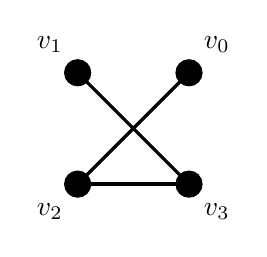
\begin{tikzpicture}
    \foreach \a in {0, 1,...,3}
        {\node[shape=circle,draw=black, fill = black] at (\a*90+45:1){};
        \node at (\a*90+45:1.5){$v_{\a}$};}
    
    \draw [draw=black,-,very thick] (45:1) to  (45+180:1);
    \draw [draw=black,-,very thick] (45+90:1) to  (45-90:1);
    \draw [draw=black,-,very thick] (45+180:1) to  (45-90:1);

    \end{tikzpicture}
       
&        
        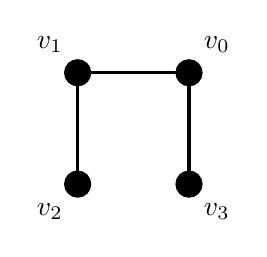
\begin{tikzpicture}
    \foreach \a in {0, 1,...,3}
        {\node[shape=circle,draw=black, fill = black] at (\a*90+45:1){};
        \node at (\a*90+45:1.5){$v_{\a}$};}
    
    \draw [draw=black,-,very thick] (45:1) to  (45-90:1);
    \draw [draw=black,-,very thick] (45:1) to  (45+90:1);
    \draw [draw=black,-,very thick] (45+90:1) to  (45+180:1);

    \end{tikzpicture}

\\
    Graph $T$  &   Graph $T'$\\
        
    \end{tabular}
    
    \vspace{1em}
    
    Notice also that $T$ and $T'$ are isomorphic trees.
    
    \item Prove that the following statements are all equivalent.
        \begin{enumerate}
            \item $G$ is a tree, i.e., $G$ is connected and has no cycles.
            \item Every two vertices of $G$ are connected by a unique path.
            \item $G$ is connected and $\lvert V \rvert = \lvert E \rvert + 1 $
            \item $G$ is a minimally connected graph, i.e., every edge is a bridge.
            \item $G$ is a maximally acyclic graph, i.e., adding any edge yields a cycle.
        \end{enumerate}
        
        \underline{$(a) \Rightarrow (b)$}
        
        Let $v, w$ be two vertices of a graph $G$ that satisfies the conditions of (a). Since $G$ is connected, then there exists a path $P = (v_0 = v, v_1, \ldots , v_k = w)$. Assume by contradiction that there exists a path $P' = (w_0 = v, w_1, \ldots, w_r = w)$ that is different to $P$. 
        
        Since both paths start at $v$, but are different paths, there exists a minimal integer $i<r$ such that $(v_0, \ldots, v_i) = (w_0, \ldots, w_i)$, but $v_{i+1} \neq w_{i+1}$. Since path $P'$ ends in $w_r=w$ and $w_r = v_k \in P$, then there exists  a minimal integer $j$ such that $j>i$ and $w_j \in V(P)$. Since $P$ and $P'$ are equal up to $i$, and both are paths, there is unique $s>i$ such that $v_s = w_j$.
        
        Notice that $(v_i, v_{i+1}, \ldots, v_s = w_j, w_{j-1}, \ldots, w_i)$ is a cycle. Since $P$ is a path, then there are no repeated vertices between $(v_i,v_{i+1}, \ldots, v_s)$. Notice that since $P'$ is also a path, there are no repeated vertices between $(w_j, w_{j-1}, \ldots, w_i)$. Notice also that from $(w_j, w_{j-1}, \ldots, w_i)$, only vertex $w_j \in P$ since $j$ is minimal with that property and also greater than $i$. It follows then that the only repeated vertex is $v_i$. Therefore $(v_i, v_{i+1}, \ldots, v_s = w_j, w_{j-1}, \ldots, w_i)$ is a cycle which contradicts condition (a). It follows from the contradiction that there must be a unique path $P$ that connects vertex $v$ to vertex $w$.
        
        \underline{$(b) \Rightarrow (c)$}
        
        Let $G$ be a graph that satisfies (b). If $\vert V \vert = 1$ then there are no edges and condition (c) holds. If $\vert V \vert = 2$ then there is only $1$ edge and $2$ vertices, therefore condition (c) holds.
        
        Lets assume that $G$ is a connected graph with at least $3$ vertices, then there exists a vertex $v$ such that $\delta(v) > 1$. Assume by contradiction that $\delta(v) = 1$ for all vertices of $G$. Consider a vertex $v_0$, since $\delta (v_0) = 1$, there exists $v_1$ adjacent to $v_0$. Since $\delta (v_1) = 1$, then it is only adjacent to $v_0$. From hypothesis, there must exist a vertex $v_2$ different from both $v_0$ and $v_1$. Since $v_0$ is only adjacent to $v_1$ and $v_1$ is only adjacent to $v_0$, any path that reaches $v_0$ consists only of vertices $v_0$ and $v_1$. Therefore, there does not exist a path from $v_2$ to $v_0$.
        
        Notice that if condition $(b)$ holds, then there exists at least one vertex $v$ such that $\delta (v) = 1$. Assume by contradiction that for all vertices in $G$, $\delta(v) \geq 2$. Consider a maximal length path $P = (v_0, v_1, \ldots, v_m)$. Since $\delta(v_m) \geq 2$, there exists a vertex $w \neq v_{m-1}$ such that $w$ is adjacent to $v_m$. Notice that $w \in P$, otherwise $P' = (v_0, \ldots, v_m, w)$ is a path of a longer length than $P$. Since $w \in P$, and $w \neq v_{m-1}$, then $w= v_i$ with $i< m-1$. $(v_i, v_{i+1}, \ldots, v_{m-1}, v_m)$ is a different path from $v_i$ to $v_m$ than $(v_i,v_m)$. This contradicts the hypothesis from $b$.
        
        Assume by (strong) induction on $\vert V \vert $ that (c) holds for graphs that satisfy (b) and such that $\vert V \vert < k$, for a fixed $k \geq 3$
        
        Let $G$ be a graph that satisfies (b) with $\vert V \vert = k $. Since we have shown that any graph that satisfies (b) has at least one vertex of degree 1, then $L = \{ v \in V \; : \; \delta(v)=1 \} $ is not empty, and it is also different from $V$.
        
        Consider graph $G'$ the subgraph induced by $V \setminus L$. Since $G'$ is a subgraph of $G$, then we only need to show that any two vertices of $G'$ are connected by a path in order to show that (b) holds in $G'$. Notice also that since $k \geq 3$, then $V\setminus L \neq \varnothing$.
        
        Let $v$ and $w$ be two vertices in $G'$, since they are also vertices in $G$, there exists a path $P = (v_0 = v, v_1, \ldots, v_m = w)$ in $G$. Notice that for all $0<i<m$, $v_i \notin L$ since $P$ is a path and $v_i$ is adjacent to both $v_{i-1}$ and $v_{i+1}$. Therefore $P$ is also a path in $G'$. Therefore condition (b) holds in $G'$. However since $L \neq \varnothing$, then $G'$ is a graph that satisfies (b). It follows from induction hypothesis that $\vert V(G')\vert = \vert E(G') \vert +1$.
        
        Since we removed vertices of degree 1, then we removed the same amount of edges and vertices. It follows that $\vert V (G) \vert - \vert V(G') \vert = \vert E(G) \vert - \vert E(G') \vert$. By substitution, we get that $ \vert V (G) \vert - (\vert E(G') \vert +1) = \vert E(G) \vert - \vert E(G') \vert$. By rearranging this equation, we get that $\vert V(G) \vert = \vert E(G)\vert +1$.
        
        This completes the induction and the proof.
        
        \vspace{1em}
        
        \underline{$(c) \Rightarrow (d)$}
        
        For a graph with one vertex (c) holds, and by vacuity (d) holds as well.
        
        Consider a graph with two vertices and one edge, then (d) holds.
        
        Let $G$ be a graph that satisfies (c) and such that it has more than 3 vertices. Then there exists a vertex $v$ such that $\delta(v) > 1$. Suppose by contradiction that all vertices have degree 1, then it follows from the handshaking lemma that $\vert E \vert = n/2$. However for $n \geq 3$ it follows that $n-1 > n/2$.
        
        Assume by induction on the number of vertices that for a fixed $k\geq 3$, that if a graph with less vertices than $k$ satisfies (c), then it also satisfies (d).
        
        Let $G$ be a graph that satisfies (c) such that $\vert V \vert = k$. We define $L$ and $G'$ as in the previous proof. Since we removed the same amount of vertices and edges, then $G'$ satisfies $(c)$. Recall that $V(G') \neq V(G)$ and $V(G') \neq \varnothing$. From induction hypothesis, we get that condition (d) holds in $G'$.
        
        Let $e = (v,w)$ be an edge in $G'$. Assume by contradiction that $e$ is not a bridge in $G$. Then, there exists a path $P$ from $v$ to $w$ that includes an edge from $G$ and that is not in $G'$. It follows that $P$ includes a leaf (vertex of degree 1) as an interior vertex. This contradicts that it is a leaf.
        
        Notice that all edges in $G$ that are not in $G'$ are bridges since they disconnect a leaf. 
        
        This shows that all edges in $G$ are bridges, therefore completing the induction and the proof.
        
        \vspace{1em}
        
        \underline{$(d) \Rightarrow (e)$}
        
        Let $G$ be a minimally connected graph, and vertices $v,w \in V$ such that $(v,w) \notin E$. 
        
        Notice first that $G$ is acyclic. Assume by contradiction that $G$ includes a cycle $C= (v_0, v_1, \ldots, v_k, v_{k+1}= v_0)$. Since there are no cycles of length 2 in a simple graph, we can assume that $v_0, v_1$, and $v_k$ are pairwise different. Therefore edge $(v_0,v_1) = e \in G$ Let us now consider subgraph $G'= G \setminus e$. We will now show that $G'$ is connected.
        
        Let $v,w \in V$. Since $G$ is connected, there exists a path $P= (w_0 = v,w_1, \ldots, w_r = w)$. If $P \notin G'$, then either $v_0 = w_i$ and $v_1 = W_{i+1}$ for some $i$ or $v_1 = w_i$ and $v_0=w_{i+1}$ for some $i$. If $v_0 = w_i$ and $v_1= w_{i+1}$ then $P'=(w_0,w_1, \ldots, w_i=v_0,v_k, v_{k-1}, \ldots v_1=w_{i+1}, \ldots, w_r=w)$ is a path in $G'$ from $u$ to $v$. If $v_1= w_i$ and $v_0 = w_{i+1}$, then $(w_0 = v,w_1, \ldots, w_i = v_1, v_2, v_k, v_{k+1}=v_0 = w_{i+1}, w_{i+2}, \ldots, w_r = w)$ is a path in $G'$ that connects $u$ to $w$. This contradicts that $G$ is minimally connected. Therefore $G$ is acyclic.
        
        Now we will show that $G$ is maximally acyclic. Assume by contradiction that $G$ is not maximally acyclic, then there exist vertices $v,w$ such that $(v,w) \notin E$ and $G \cup (v,w)$ is still acyclic. Since $G$ is connected, there exists a path $P=(v_0 = v, v_1, \ldots, v_k = w)$ that connects $v$ to $w$. Notice that $C= (v_0 = v, v_1, \ldots, v_k = w, v_0)$ is a cycle. Therefore $G$ is minimally acyclic.
        
        This completes the proof.
        
        \vspace{1em}
        
        \underline{$(e) \Rightarrow (a)$}
        
        Let $G$ be a maximally acyclic graph. Notice that $G$ does not include cycles.
        
        Now we will show that $G$ is connected. Let $v,w$ be two vertices of $G$, if $(v,w) \in E$ then $(v,w)$ is a path from $v$ to $w$. Now let us assume that $e=(v,w) \notin E$. Notice then that $G \cup e$ produces a cycle $C = (v_0=v, v_1=w, \ldots, v_k, v_{k+1}= v)$ that includes edge $e$. Notice that $P=(v=v_{k+1},v_k, v_{k-1}, \ldots,v_1)$ is a path that connects $v$ to $w$ that does not include edge $e$. Therefore $P \in G$, and thus $G$ is connected.
        
        This completes the proof cycle and therefore it completes the proof for equivalence.
        
        \item Show that every graph with at least as many edges as vertices contains a cycle.
        \vspace{1em}
        
        Let $G_1, G_2, \ldots, G_k$ be the connected components of $G$, and $V_1,V_2, \ldots, V_k$ and $E_1,E_2, \ldots, E_k$ their sets of vertices and edges respectively. Then there exists a connected component $G_i$ such that $\vert V_i \vert \leq \vert E_i \vert$. Assume by contradiction that for all $i$, $\vert V_i \vert < \vert E_i \vert$. It follows that $\displaystyle\sum\limits_{i=1}^{k} \vert V_i \vert = \vert V \vert < \displaystyle\sum \limits_{i=1}^{k} \vert E_i \vert = \vert E \vert$. This contradicts the hypothesis. Therefore, there exists a connected component of $G$, $G_i$ such that $\vert V_i \vert \leq \vert E_i \vert$.
        
        Since $G_i$ is connected and $\vert V_i \vert \leq \vert E_i \vert$, then $G_i$ a minimally connected graph $G_i'$. Since $\vert V_i\vert \neq \vert E_i \vert + 1$, then $G_i$ is not minimally connected, and therefore $G_i'$ is a proper subgraph. Notice that since $G_i'$ is minimally connected, then it is also maximally acyclic. Therefore $G_i$ includes a cycle. Since $G_i$ is also a subgraph of $G$, then $G$ includes a cycle.
        
        \item Let $T$ be a tree without vertices of degree $2$. Show that $T$ has more leaves than internal nodes using the handshaking lemma.
        \vspace{1em}
        
        Assume by contradiction that there are at least the same amount of internal nodes as leaves. Then $\displaystyle\sum\limits_{v\in V}\delta(v)\geq 3 \cdot (n/2) + (n/2) = 2 \cdot n$. This implies that there are at least $n$ edges (via the handshaking lemma). This contradicts that $T$ is a tree.
        
        \item Let $G$ be a graph with at least two vertices. Prove or disprove.
        
        \begin{enumerate}
            \item Deleting a vertex of maximal degree $\Delta$ cannot increase the average degree.
            
            Consider a vertex $v_0$ such that it increases the average degree when deleted. Let $G' = G \setminus v_0$
            
            Notice that the following equations hold:
            
            \begin{equation}
             Ad(G) = \displaystyle\left(\sum\limits_{v\in V} \delta(v)\right) \cdot 1/n
            \end{equation}
            
            \begin{equation}
            Ad(G') = \displaystyle\left [\displaystyle\left(\sum\limits_{v\in V} \delta(v)\right)-2\cdot \delta(v_0) \right ] \cdot 1/(n-1)
            \end{equation}
            
            Notice from hypothesis that $Ad(G)< Ad(G')$, therefore, the following inequality holds
            
            \begin{equation}
                (n-1) \cdot \displaystyle \left ( \sum \limits_{v \in V}\delta(V) \right )< n \cdot \displaystyle \left ( \sum \limits_{v \in V} \delta(v) \right)-2n \cdot \delta(v_0)
            \end{equation}
            Inequality (3) rearranges into the following inequality
            
            \begin{equation}
                2 \cdot \delta(v_0) < Ad(G)
            \end{equation}
            
            This implies that $\delta(v_0)$ should be less even than half the average. Therefore $v_0$ cannot be of maximal degree.
            
            This proves that statement (a) is true.
            \item Deleting a vertex of minimal degree $\delta$ cannot decrease the average degree.
            
            False.
            
            Consider the graph $G$ with vertices $v_0,v_1$ and only edge $(v_0,v_1)$. The average degree of $G$ is 1, the minimal degree is also $1$. Now consider $G' = G \setminus v_1$. $G'$ is the graph with only one vertex. The average degree of $G'$ is $0$.
            
            One may also consider a length 2 path. It has an average degree of $4/3$. If we remove a vertex of minimal degree, then we have a path of length 1 which has an average degree of $1< 4/3$
        \end{enumerate}
        
        \item Let $G_n$ be the graph whose vertices are the permutations of $\{1,2,\ldots, n \}$. Two vertices in $G_n$ are adjacent if they differ by swapping two numbers next to each other. Show that $G_n$ is connected.
        
        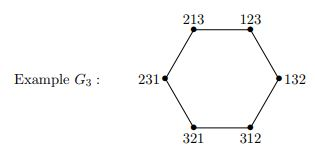
\includegraphics[width=0.5\textwidth]{perm.JPG}
        
        \vspace{3em}
        
        We will proceed by induction over $n$.
        
        Notice that $G_1$ is the graph with only one vertex, and it is connected. Notice also that $G_2$ is the graph with 2 vertices $1,2$ and $2,1$ and from definition $[(2,1), (1,2)] \in E(G_n)$. Therefore it is connected.
        
        Lets assume by induction that $G_k$ is connected for a fixed $k$. Let $G_{k+1}$ be the permutation graph for $k+1$. We will show a path from $w=(1,2,\ldots,k+1)$ to any vertex $(v_1,v_2, \ldots,v_{k+1})$, where each $v_i = j$ for some $j \in \{1,\ldots ,k+1\}$
        
        Let $v=(v_1,v_2, \ldots,v_{k+1})$. Since $v$ is a permutation, then there exists $i$ such that $v_i = 1$. Let us consider vertex $v'= (1, v_2,v_3, \ldots, v_{i-1},v_1,v_{i+1}, \ldots, v_k)$. Notice that $v$ is adjacent to $v'$, since there is a swap, namely $v_i$ for $v_1$, that produces $v'$ from $v$.
        
        Consider the following induced subgraph of $G_{k+1}$, $G_{1,k}$, with set of vertices $V(G_{1,k})= \{ (w_1,w_2, \ldots,w_k, w_{k+1}) \in V(G_{k+1}) \quad : \quad w_1 = 1 \}$.
        
        We will show that $G_{1,k}$ is isomorphic to $G_k$.
        
        Consider the following vertex map $\mu: V(G_{1,k}) \rightarrow V(G_k)$
        $\mu[ (1,w_2, w_3, \ldots, w_{k+1}) ] = (w_2-1, w_3-1, \ldots, w_i -1, \ldots, w_{k+1}-1)$. Notice that $\mu $ is bijective, since all $w_i$ for $i \geq 2$ are different pairwise positive integer values from $2$ to $k-1$.
        
        Let $x,y \in V(G_{1,k})$ be two adjacent vertices in $G_{1,k}$, $x = (1,x_2,x_3, \ldots,x_{k+1})$. Since $y$ is adjacent to $x$, there exist $i,j$ such that $$y = (1,x_2, \ldots, x_{i-1}, x_j, x_{i+1}, \ldots, x_{j-1}, x_j, x_{j+1}, \ldots x_{k+1})$$
        
        Notice that $\mu(x) = (x_2-1,x_3-1,\ldots, x_{k+1}-1)$ and $$\mu(y)= (x_2-1, \ldots, x_{i-1}-1, x_j-1, x_{i+1}-1, \ldots, x_{j-1}-1, x_j-1, x_{j+1}-1, \ldots x_{k+1}-1)$$
        
        Since $G_k$ is the permutation graph for $k$, then $\mu(x)$ is adjacent to $\mu(y)$.
        In a symmetrical way, the inverse map of $\mu$, $\mu^{-1}(z_1,z_2, \ldots, z_k) = (1,z_1+1,z_2+1 \ldots, z_k+1)$ also maps edges to edges.
        
        Therefore $\mu$ is a graph isomorphism and therefore $G_{1,k}$ is isomorphic to $G_k$.
        
        It follows from induction that $G_k$ is connected, therefore $G_{1,k}$ is also connected.
        
        Now notice that both $v',w \in V(G_{1,k}$. It follows that there exists a path $P$ from $v'$ to $w$ in $G_{1,k’}$. Since it is a subgraph of $G_{k+1}$ then $P' = (v,v') \cup P$ is a path in $G_{k+1}$ . Therefore $G_{k+1}$ is connected.
        
        This completes the induction and the proof.
        
        
        
        
        
\end{enumerate}

\end{document}